\documentclass[a4paper,12pt]{report}
\usepackage{alltt, fancyvrb, url}
\usepackage{graphicx}
\usepackage[utf8]{inputenc}
\usepackage{float}
\usepackage{hyperref}
\usepackage{csquotes}
\usepackage[style=verbose-ibid,backend=bibtex]{biblatex}
\usepackage[italian]{babel}
\usepackage[italian]{cleveref}
\usepackage{xurl}

\title{%
  IoT Assignment 2 \\
  \large Smart bridge}

\author{Mattia Panni \\ Riccardo Fiorani \\ Eleonora Falconi \\ Alesja Delja}
\date{\today}

\begin{document}
\maketitle
\tableofcontents


\chapter{Design}
In questa sezione verranno spiegate le scelte di design intraprese, in una prima fase di interazione fra i membri del gruppo, e che ci hanno permesso, dopo una raffinazione successiva, di arrivare alla soluzione finale del sistema.
\section{Architettura}
Vengono di seguito riportate le scelte di massima prese in fase di progettazione del sistema.
\subsection{Macchine a stati finiti (FSM)}
Durante una prima iterazione, a seguito della lettura del documento, abbiamo deciso di creare due macchine a stati finiti, una per ognuno dei seguenti macro task
\begin{enumerate}
    \item \textbf{Smart Lightining System}. Sistema di controllo per il lampione. Tale task il compito di accendere il lampione, qualora la luce ambientale fosse sotto una certa soglia (threshold) e venissero rilevate persone sul ponte e che lo spegnesse in assenza di queste, da almeno 5 secondi. Va ovviamente mantenuto spento nel caso in cui la luce rilevata fosse sopra la soglia, indipendentemente dalla presenza o meno di persone.
    \item \textbf{Smart Water Control System}. Sistema che, sulla base del livello raggiunto dall'acqua, aprisse o meno una valvola.
\end{enumerate}
\subsubsection{Smart Lightning System}
La macchina a stati finiti pensata per questo macro sistema è rappresentata in figura \ref{fig:FSMSmartLightning}.

Il diagramma si compone di due stati 
\begin{itemize}
    \item \textbf{ON}. Rappresenta lo stato in cui il lampione è acceso. Da qualsiasi punto dello schema, entrando in questo stato, il lampione (nell'immagine $L_{A}$) dev'essere acceso. 
    \item \textbf{OFF}. È lo stato di spegnimento del lampione. Così come per ON, anche in questo caso la voce ``entry / $L_{A} =$ off'' rappresenta il fatto che da qualsiasi stato si entri, la prima istruzione da eseguire è quella di spegnere il lampione. Come mostra l'immagine, l'ingresso avviene in questo stato, pertanto all'avvio del sistema il lampione risulterà spento.
\end{itemize}
La transizione da OFF ad ON si verifica qualora si verifichi l'evento di passaggio di persone sul ponte (in figura P), la cui guardia è costituita dal livello di luce ambientale sotto una certa soglia ($L_S \leq TH_1$). Il viceversa, cioè da ON a OFF, avviene in due casi
\begin{itemize}
    \item Quando sul ponte non passano persone da un certo tempo $T_1$. Per modellare questo vincolo in termini di macchine a stati finiti è stato introdotto un timer (variabile t) che può essere vista come una macchina a stati finiti a se stante (mostrato in figura \ref{fig:FSMTimer}).
    \item Quando il livello di luce ambientale supera il threshold precedentemente menzionato.
\end{itemize}
Le transizioni da uno stato a se stesso vengono mostrate perché, come mostra la nota in figura, affinché sia modellato il vincolo che il lampione si spenga dopo un certo tempo da quando non ci sono persone sul ponte, al passaggio di queste il timer si deve resettare.
\begin{figure}[H]
\centering
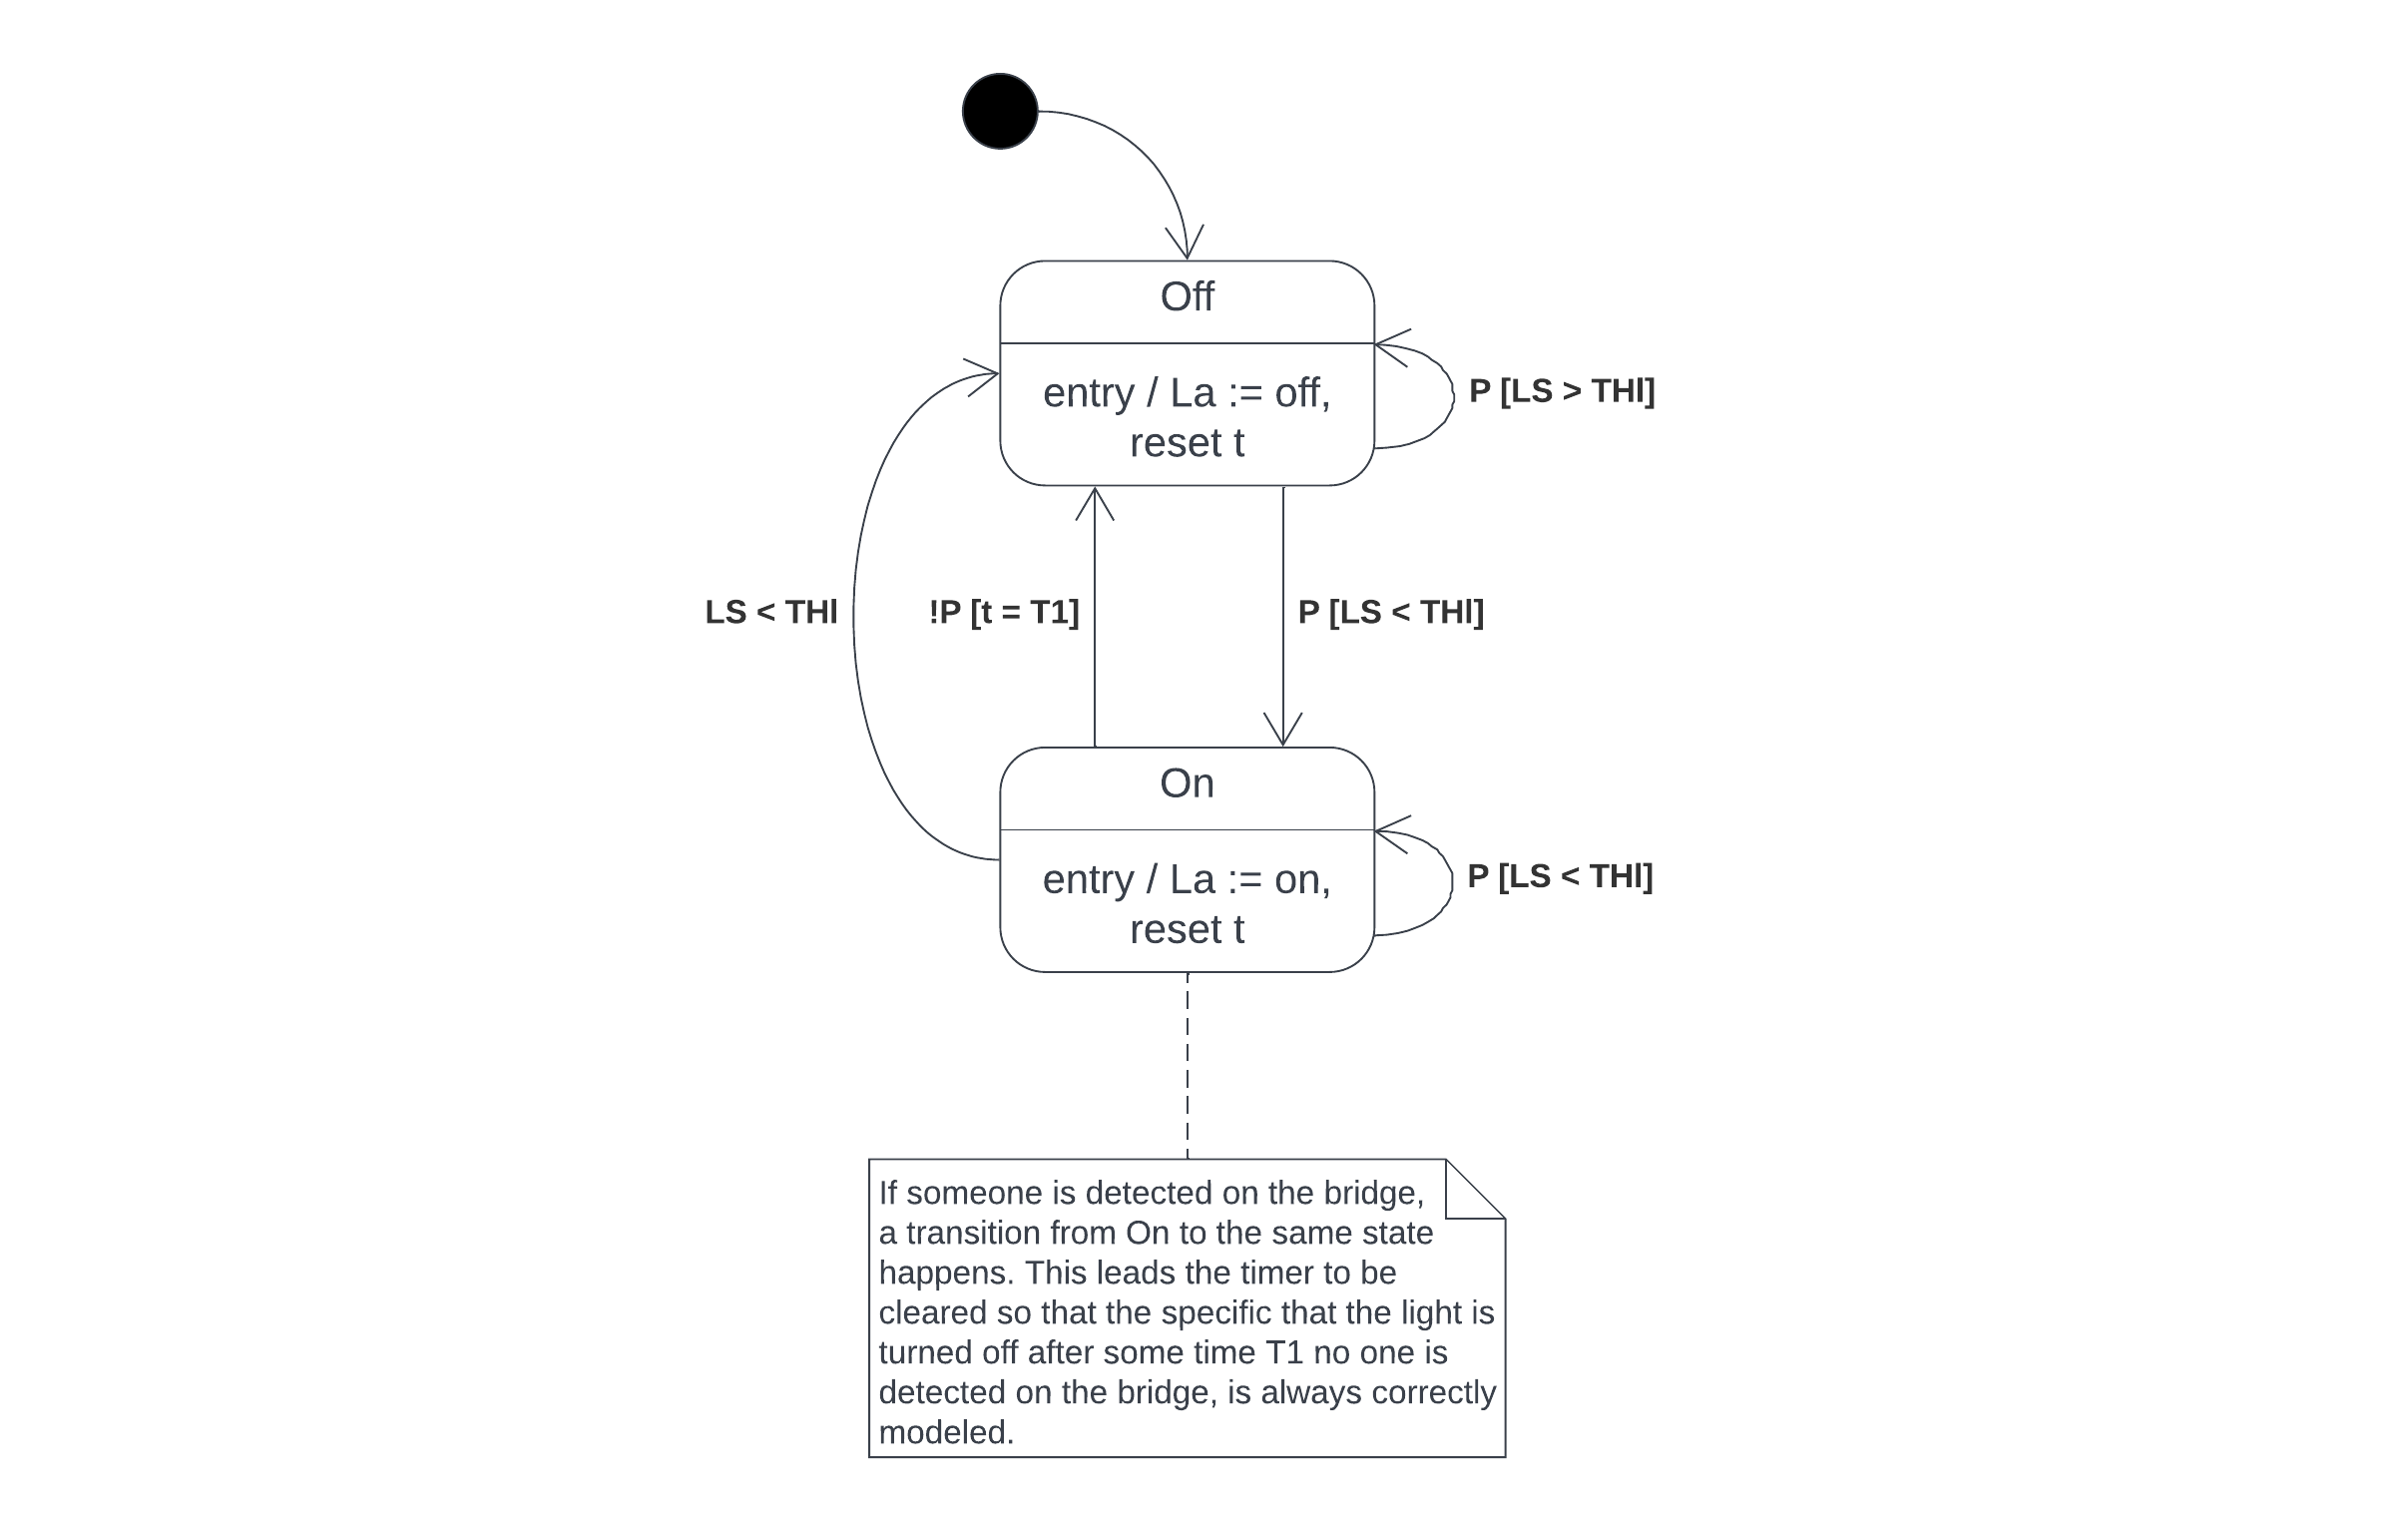
\includegraphics[width=\textwidth]{img/State - SmartLighting.png}
\caption{Smart Lightning System Finite State Machine.}
\label{fig:FSMSmartLightning}
\end{figure}

\begin{figure}[H]
\centering
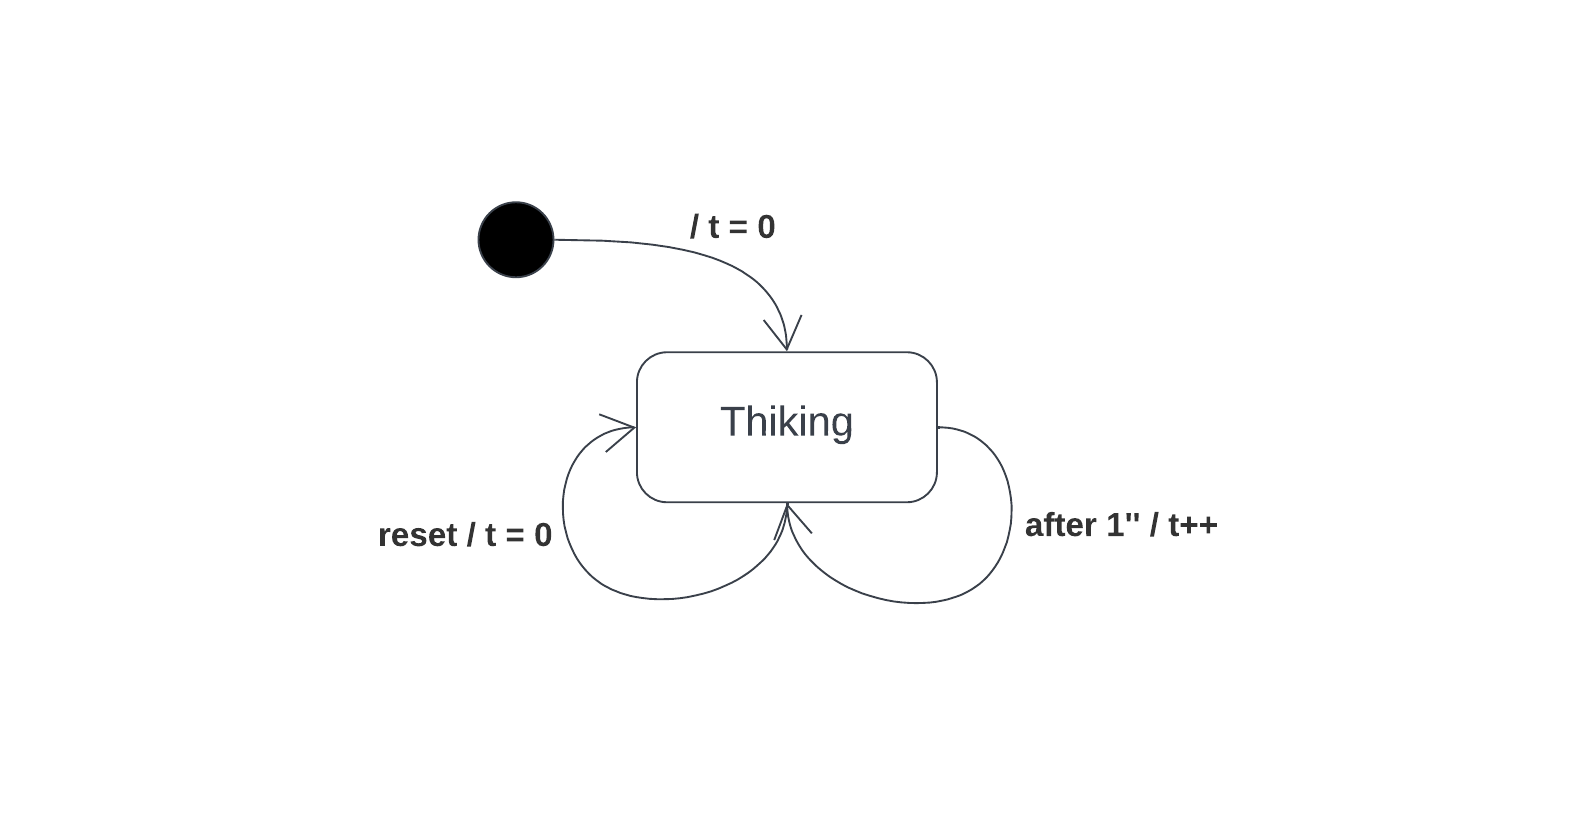
\includegraphics[width=\textwidth]{img/State - Timer.png}
\caption{Timer Finite State Machine.}
\label{fig:FSMTimer}
\end{figure}



\subsubsection{Smart Water Control System}
Come mostra la figura \ref{fig:FSMSmartWaterControl}, il sistema può trovarsi in uno dei seguenti tre stati
\begin{enumerate}
    \item \textbf{NORMAL}. In questo stato, in cui l'acqua è sotto un livello $WL_1$. In tal caso il led $L_b$ deve accendersi, $L_c$ deve rimanere spento, il servo dev'essere chiuso (0°), il display spento e il lampione $L_a$ deve comportarsi come stabilisce il macro task \emph{Light Task}.
    \item \textbf{PRE ALARM}. Si entra nello stato di pre alarm qualora l'aqua salisse entro un intervallo[$WL_1$, $WL_2$]. In esso il lampione rimane controllato dal \emph{Light Task}. Il led $L_c$ va fatto lampeggiare con un periodo di 2 secondi e il display deve mostrare \emph{solo} il livello dell'acqua. Le ultime due, a differenza dell'accensione del lampione, che costituisce un evento, sono attività ripetute nel tempo.
    \item \textbf{ALARM}. In questo stato, indipendentemente dallo stato in cui si trova \emph{Light task}, il lampione deve spegnersi. Stesso deve fare $L_b$ mentre $L_c$ deve essere acceso. La valvola dev'essere mappata in un intervallo [0°, 180°] sulla base del livello dell'acqua, compreso a sua volta in un intervallo [$WL_2$, $WL_\textrm{max}$]. Il display deve mostrare sia il livello dell'acqua che l'apertura della valvola.
\end{enumerate}
Le transizioni da uno stato all'altro sono tutte causate dall'evento di misurazione del livello dell'acqua, in figura chiamato \emph{measure water level(PE)} (il quale va fatto ad una frequenza differente (PE) a seconda dello stato in cui ci si trova) e ovviamente la guardia sarà il livello misurato.

\begin{figure}[H]
\centering
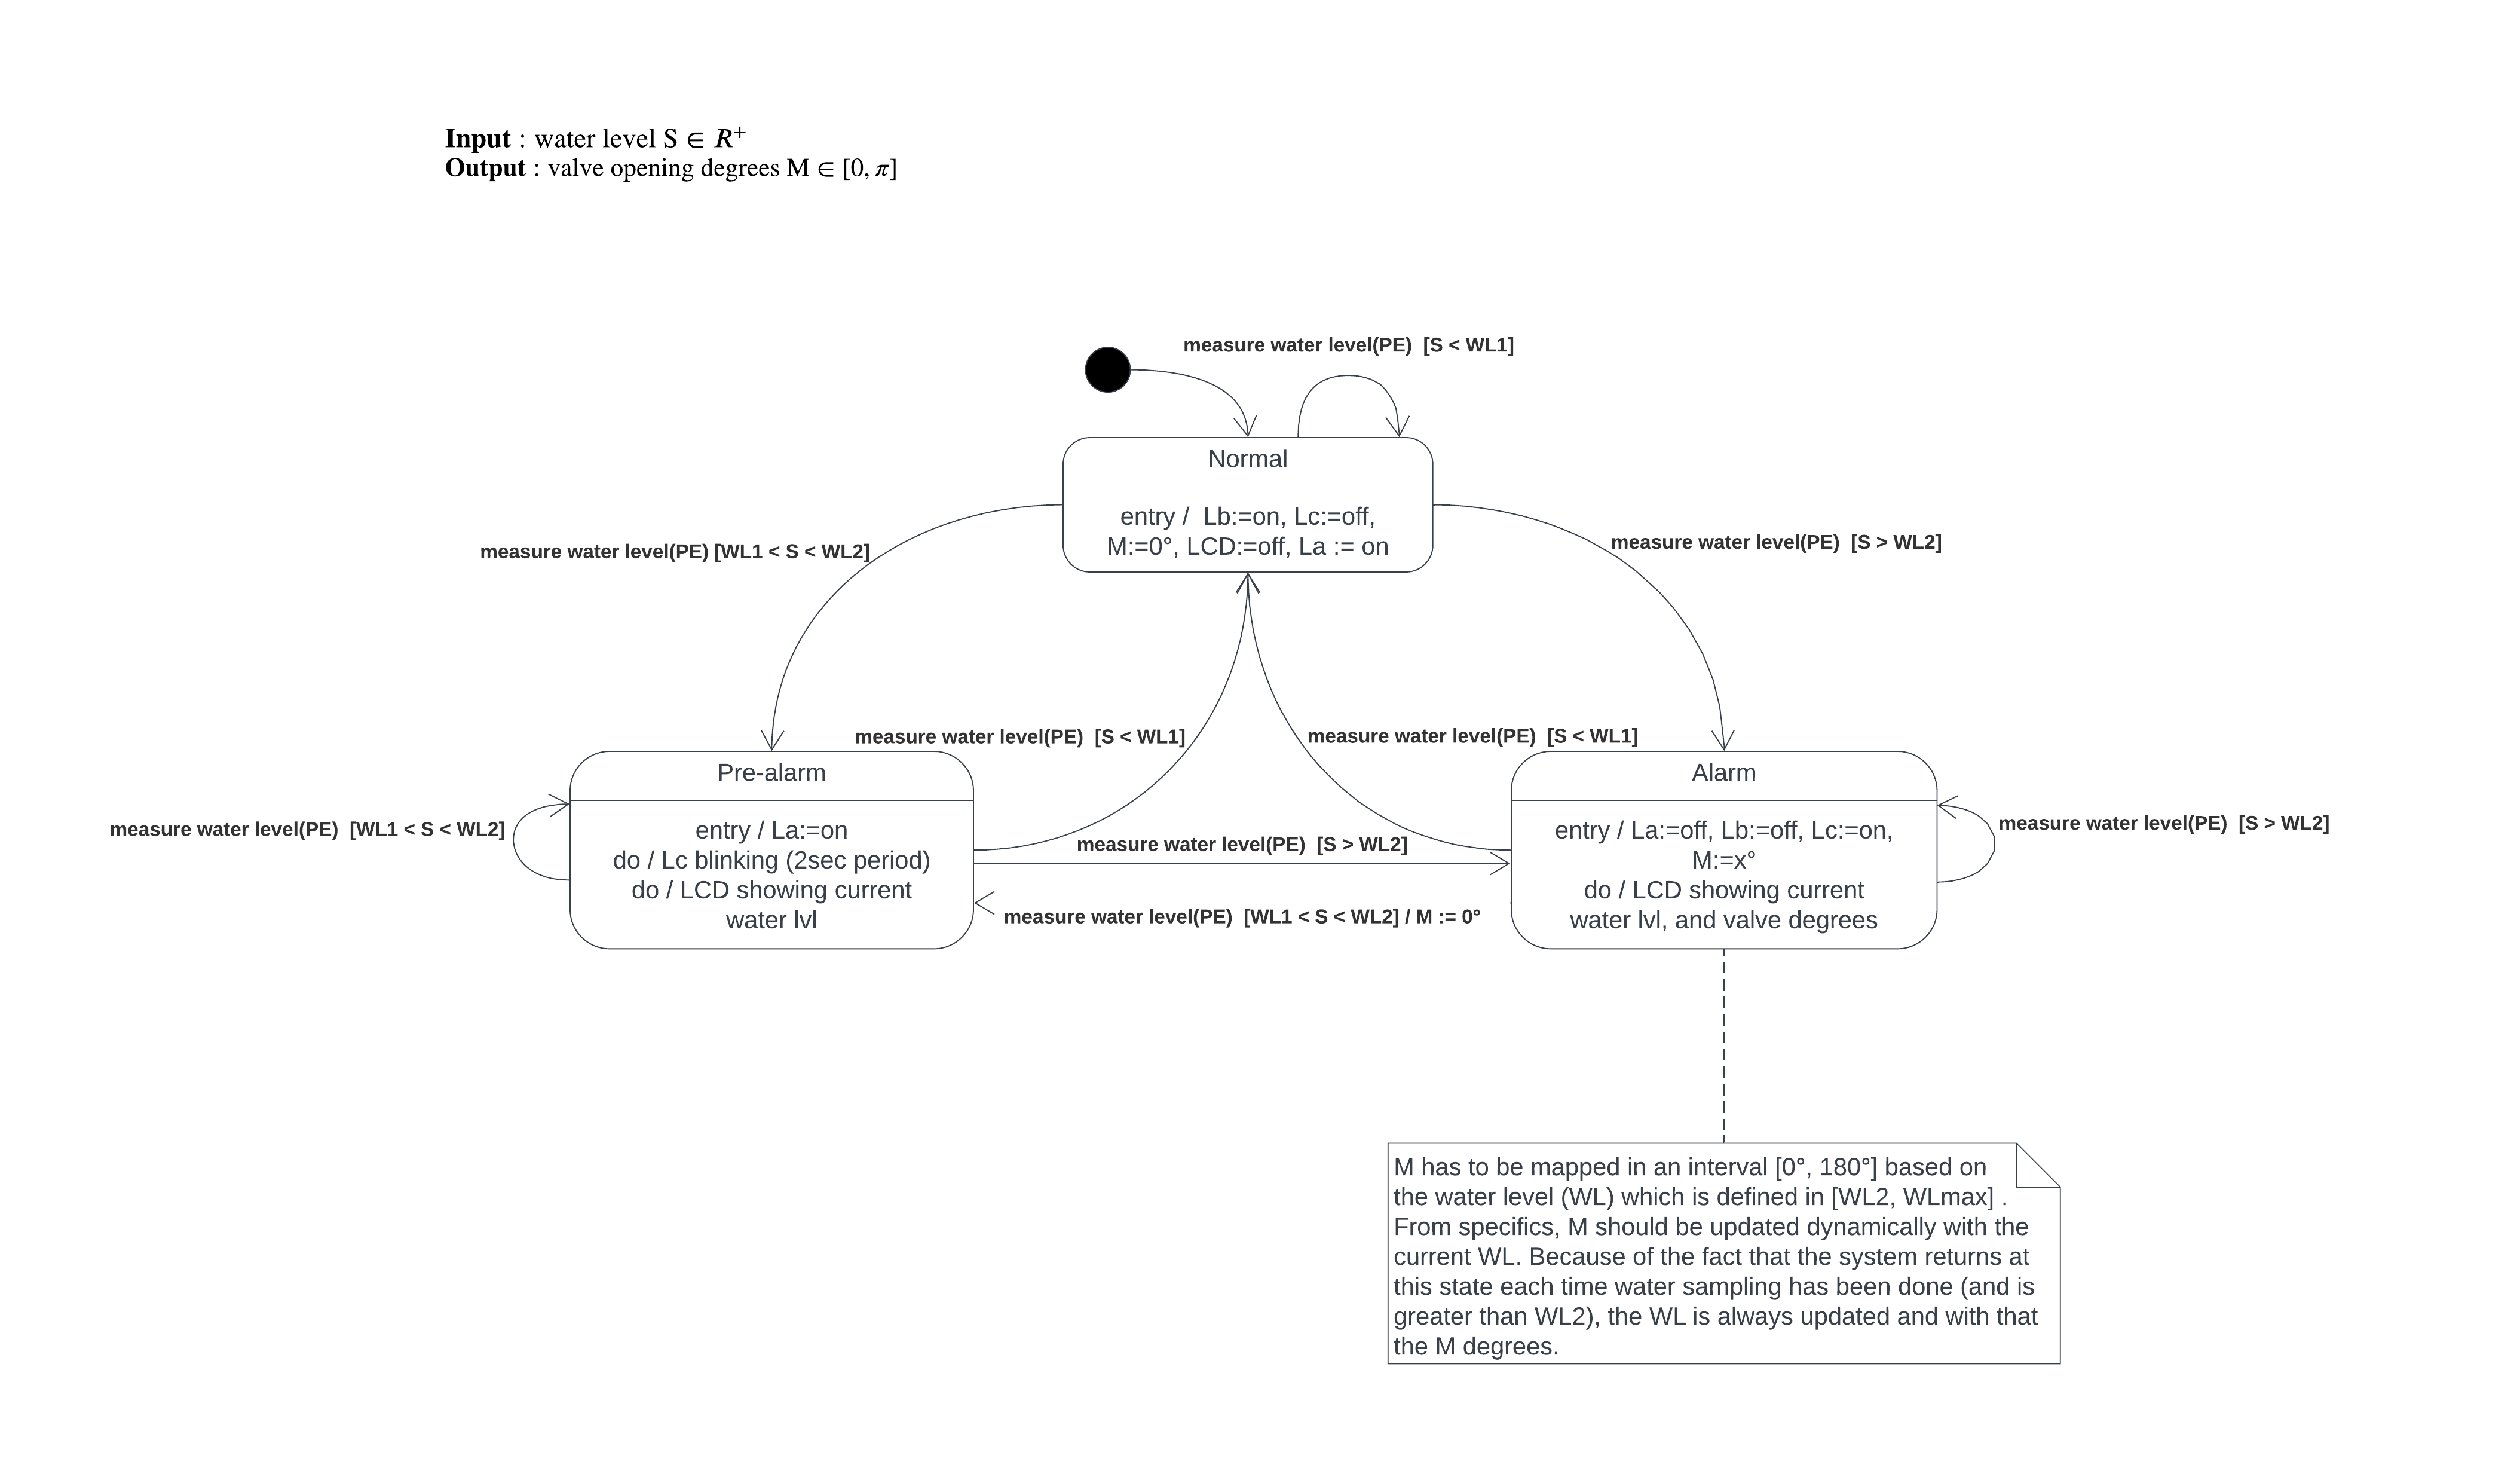
\includegraphics[width=\textwidth]{img/State - WaterLevel.png}
\caption{Smart Water Control System Timer Finite State Machine.}
\label{fig:FSMSmartWaterControl}
\end{figure}

\subsection{Diagrammi delle classi}
Dopo una prima analisi abbiamo ipotizzato di implementare le due macro attività descritte al paragrafo precedente come task. In questo modo, attraverso un sistema di scheduling round robin rendendo l'esecuzione dell'intero sistema più controllata e producendo un sistema che astraesse dal livello più ``elettronico''. 

La figura \ref{fig:classiTask}, mostra un primo abbozzo del sistema.

\begin{figure}[H]
\centering
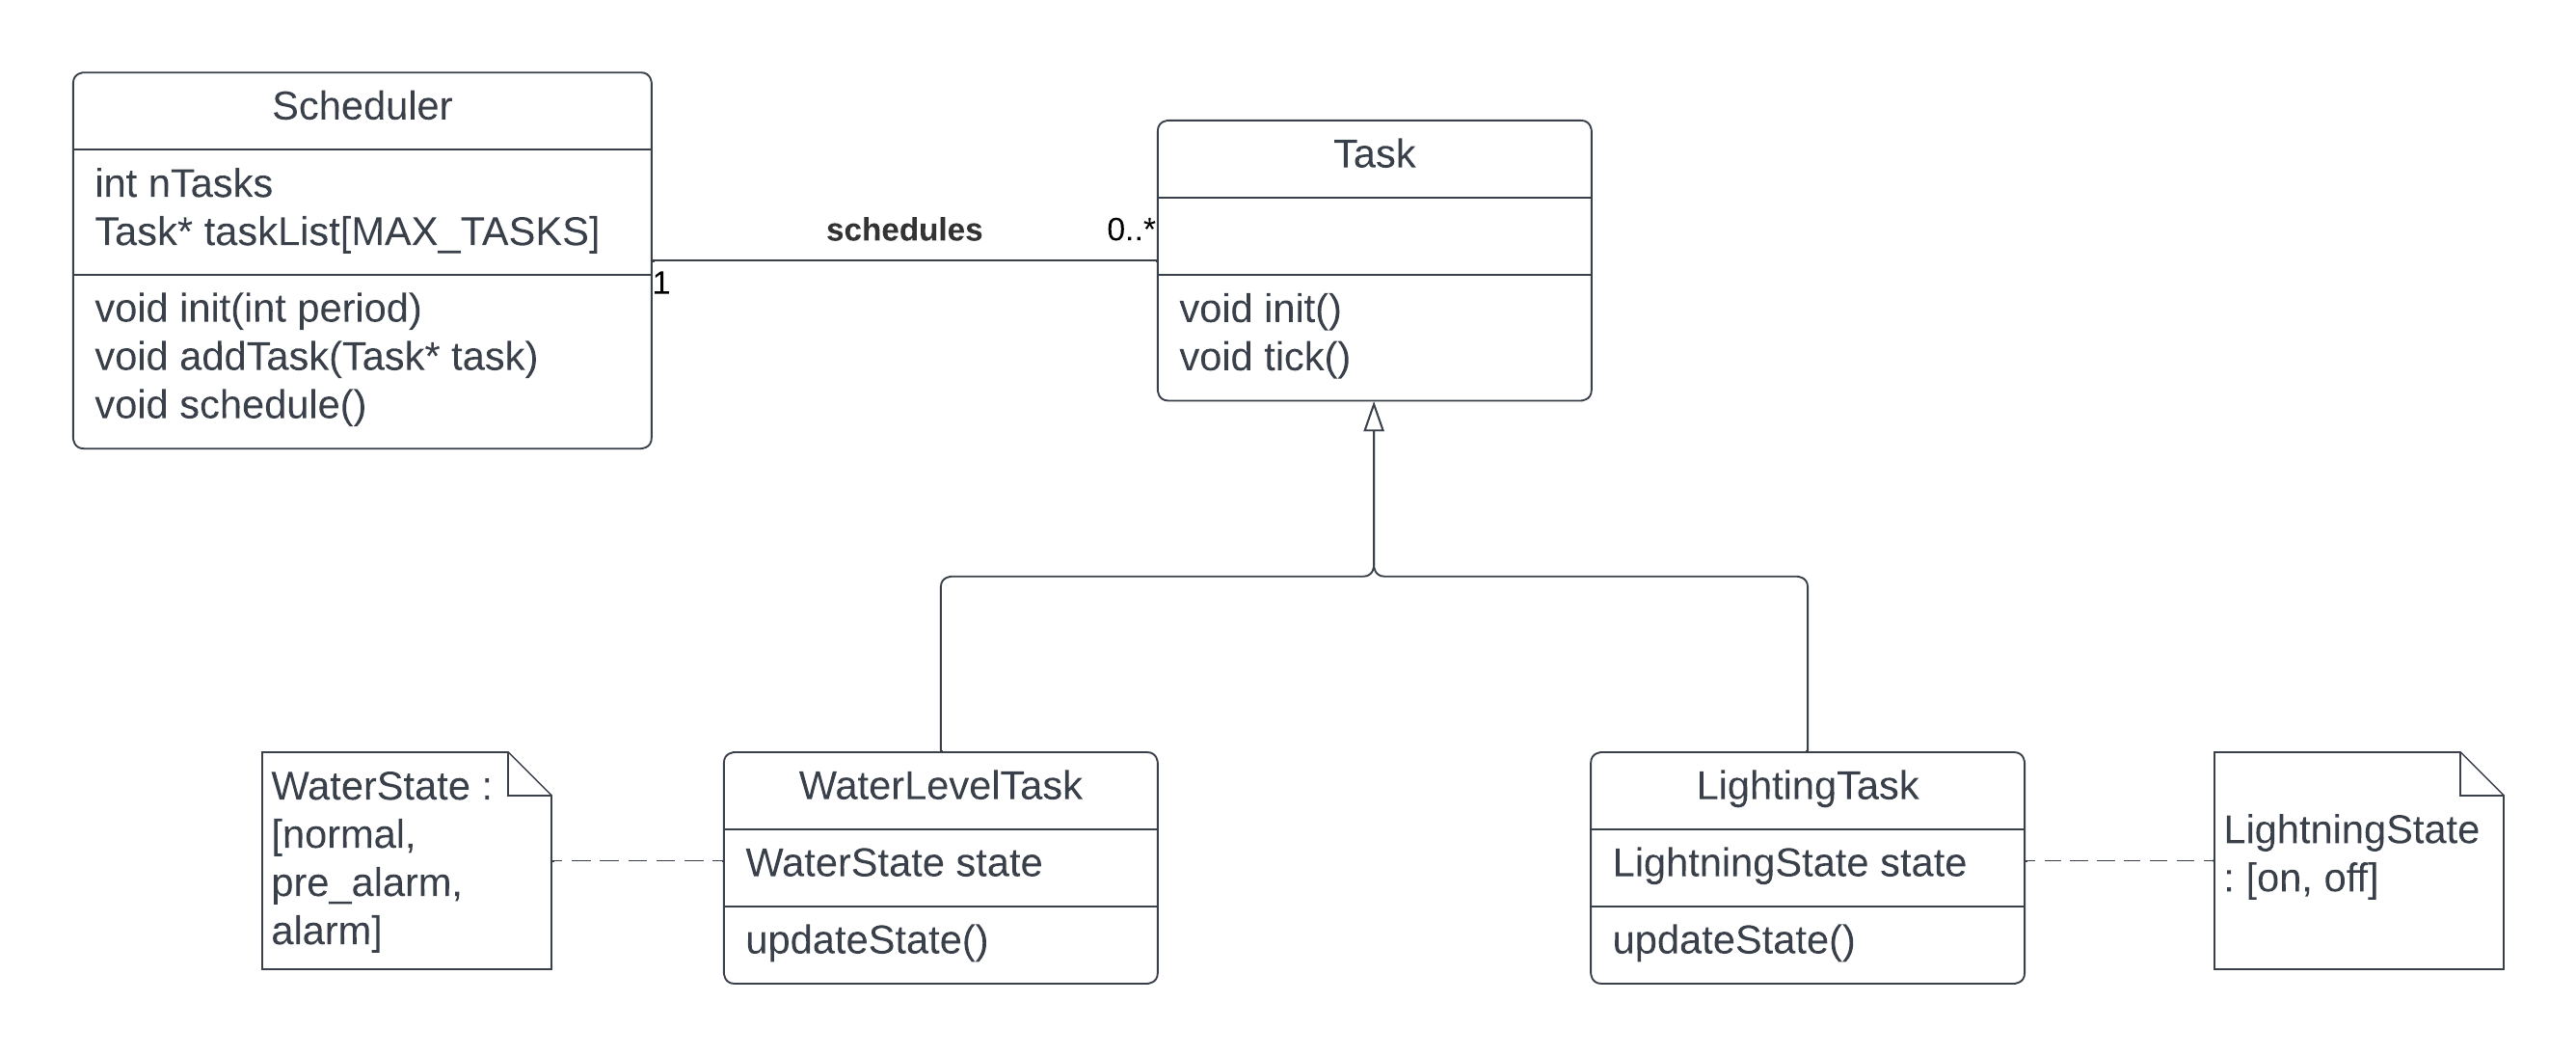
\includegraphics[width=\textwidth]{img/Classi - WaterLevelScheduling.png}
\caption{Activities as scheduled tasks.}
\label{fig:classiTask}
\end{figure}

\section{Architettura nel dettaglio}
In questo paragrafo si spiegherà nel dettaglio l'architettura implementata.
\subsection{Tasks}
Come anticipato, a seguito di iterazioni successive, siamo giunti ad una decomposizione dei macro task descritti nei paragrafi superiori. In particolare si hanno
\begin{enumerate}
    \item \textbf{Smart Water Controller Task}. Il cui funzionamento e stati rimangono invariati rispetto alla versione precedentemente descritta. Ciò che varia sono le attività che vengono internamente gestite da quest'unico task, notevolmente diminuite rispetto alla versione iniziale.
    \item \textbf{Smart Lightning Task}. Come la (1).
    \item \textbf{Sonar Task}. Poiché la misurazione del livello dell'acqua tramite sonar era un qualcosa di indipendente dalla gestione degli altri componenti interni a water task, nonché qualcosa di interesse anche per altre attività (come quella dell'accensione del lampione e della stampa sul display), abbiamo pensato di implementarla come un task autonomo. Spiegheremo in seguito come è stato possibile aggiornare la velocità di campionamento del sonar sulla base del livello d'allarme.
    \item \textbf{Servomotor Task}. Anche in questo caso, come per il sonar, concettualmente è qualcosa di indipendente al task del water level. 
    \item \textbf{Serial Comunication Task}. Task adibito alla comunicazione, tramite porta seriale, con un'interfaccia sviluppata in Java.
    \item \textbf{Lcd Screen task}. Task adibito alla rappresentazione su display (e stampa in seriale) dei dati relativi a servo motore, sonar e livello d'allarme e stato del lampione su seriale. 
    \item \textbf{Blinking Task}. Per fare in modo che il periodo di blinking dei led potesse essere indipendente dalla frequenza di campionamento del livello dell'acqua, il led $L_c$ dev'essere posto in un task separato.
    \item \textbf{Manual control task}. Task adibito all'override del controllo automatico delle valvole. Consente di controllare manualmente, mediante potenziometro, il livello di apertura del servo.
\end{enumerate}

\subsubsection{Sonar e Servomotor tasks}
Questi task sono triviali in quanto costituiti da un solo stato rispettivamente \textbf{MEASURING} per Sonar e \textbf{WRITING} per Servomotor, il quale, a seconda del dispositivo in questione registra o scrive una variabile. Per motivi di semplicità verrà mostrata solo la FSM del sonar.

\begin{figure}[H]
\centering
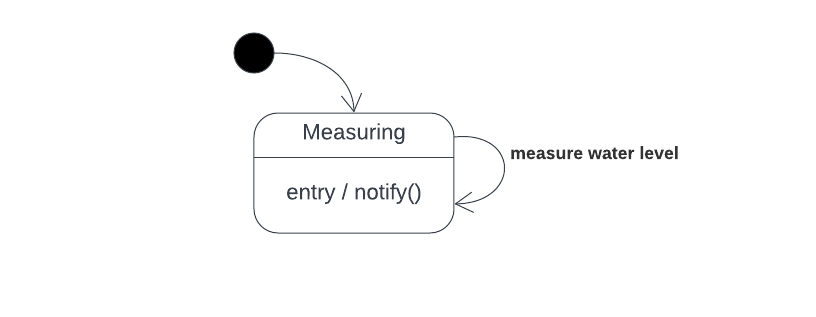
\includegraphics[width=\textwidth]{img/State - Sonar.png}
\caption{FSM Sonar task.}
\label{fig:FSMSonar}
\end{figure}

\subsubsection{Serial Comunication Task}
Ancora da definire

\subsubsection{Lcd Screen task}
Questo task si basa su quanto gli viene comunicato dagli altri task. In particolare i suoi stati mappano fedelmente quelli di Smart Water Controller poiché, a seconda del livello dell'acqua attualmente misurato (e conseguentemente del livello di allarme attivo), il display dovrà spegnersi, stampare il livello dell'acqua e il livello di apertura delle valvole o solamente il primo dei due dati. Questi dati verranno forniti da sonar task e servo task.
Poiché la transizione da ogni stato ad ogni altro è identica a quella mostrata in figura \ref{fig:FSMSmartWaterControl}, la figura \ref{fig:FSMLCDTask} ha un evento di transizione solamente su un arco.

\begin{figure}[H]
\centering
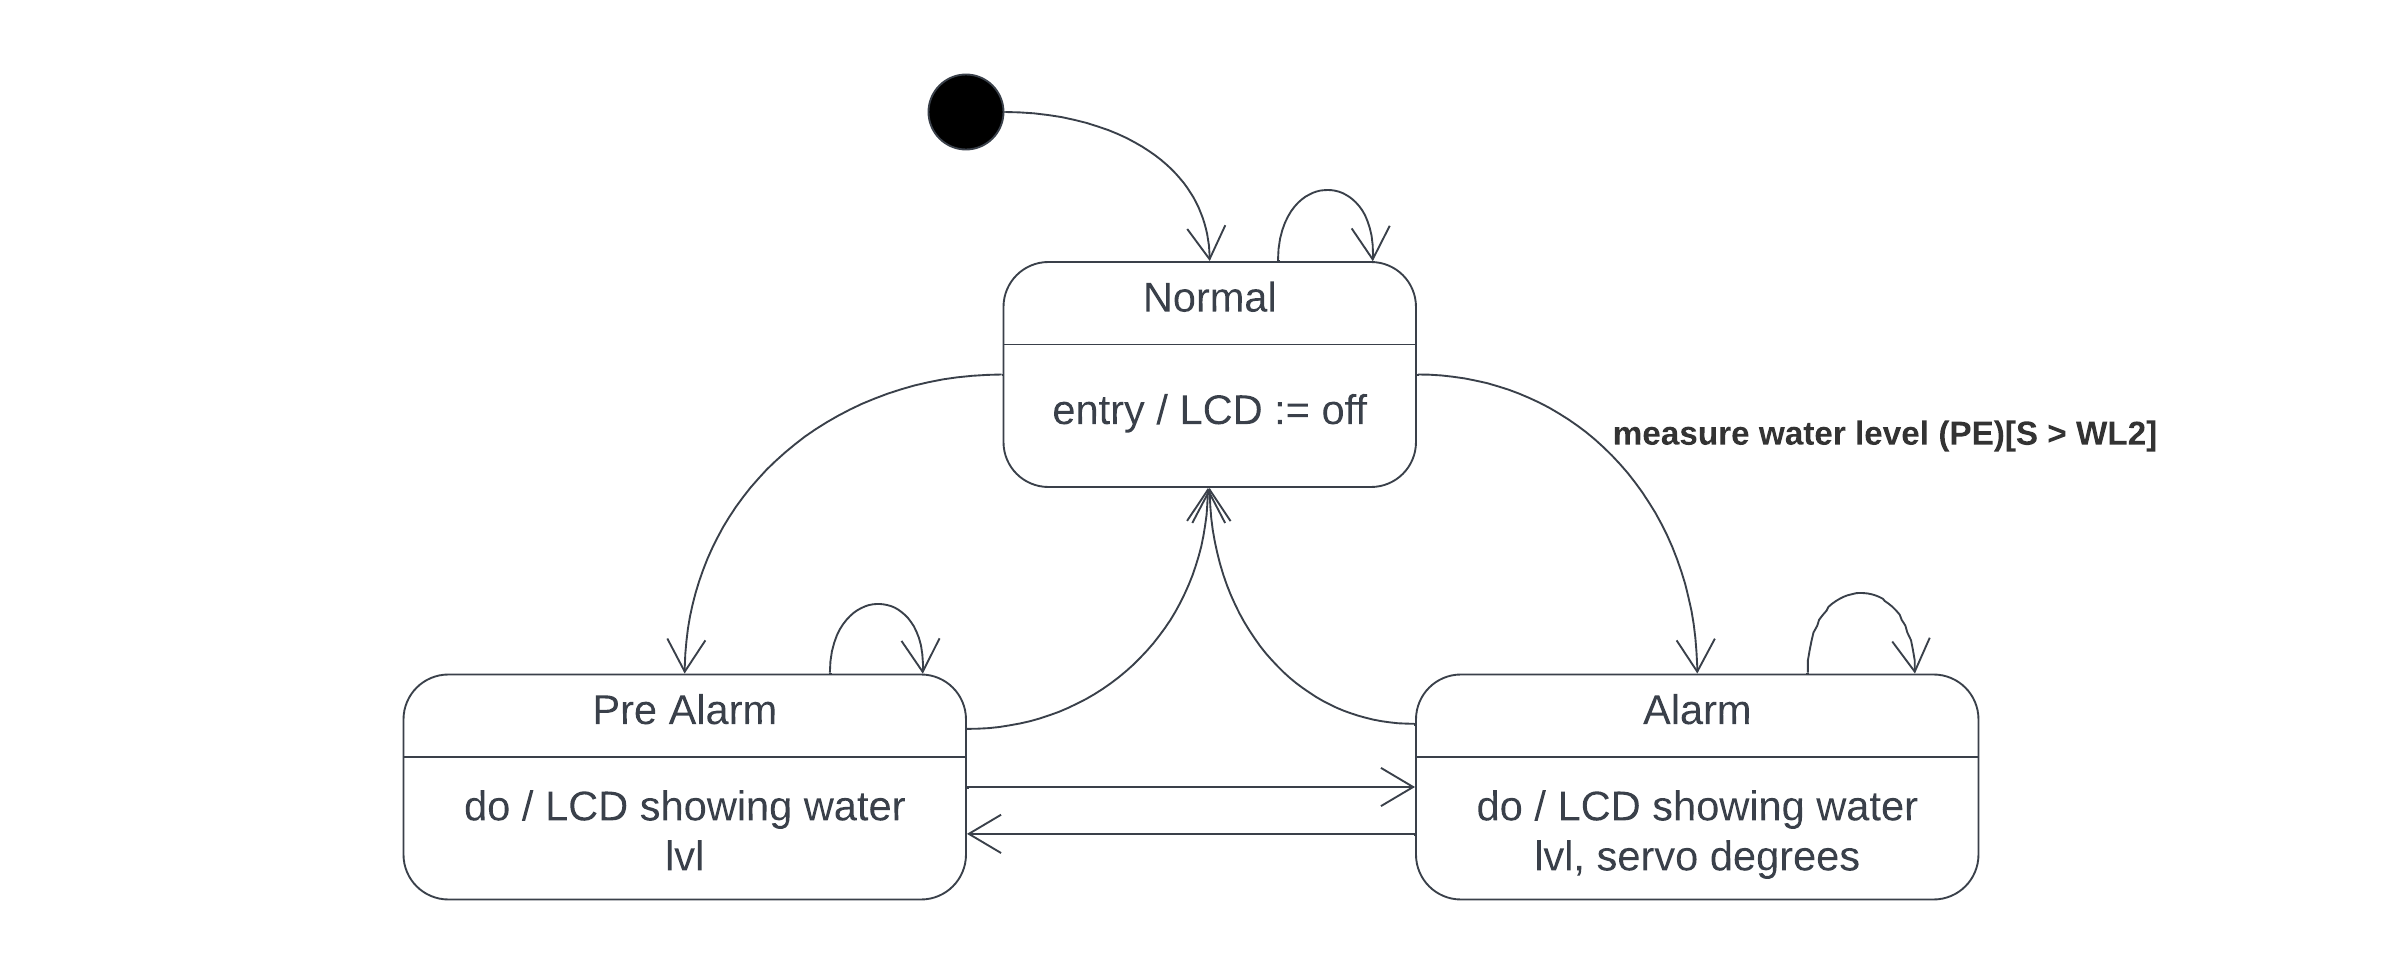
\includegraphics[width=\textwidth]{img/State - LCDScreen.png}
\caption{FSM Lcd Screen.}
\label{fig:FSMLCDTask}
\end{figure}

\subsubsection{Blinking task}
Cosi come per Screen task, anche in questo caso gli stati sono esattamente quelli di water task. Sulla base di questi, il led dovrà blinkare, rimanere acceso o spento. Per quanto riguarda gli eventi che fanno transitare di stato vale il discorso fatto su lcd task.

\begin{figure}[H]
\centering
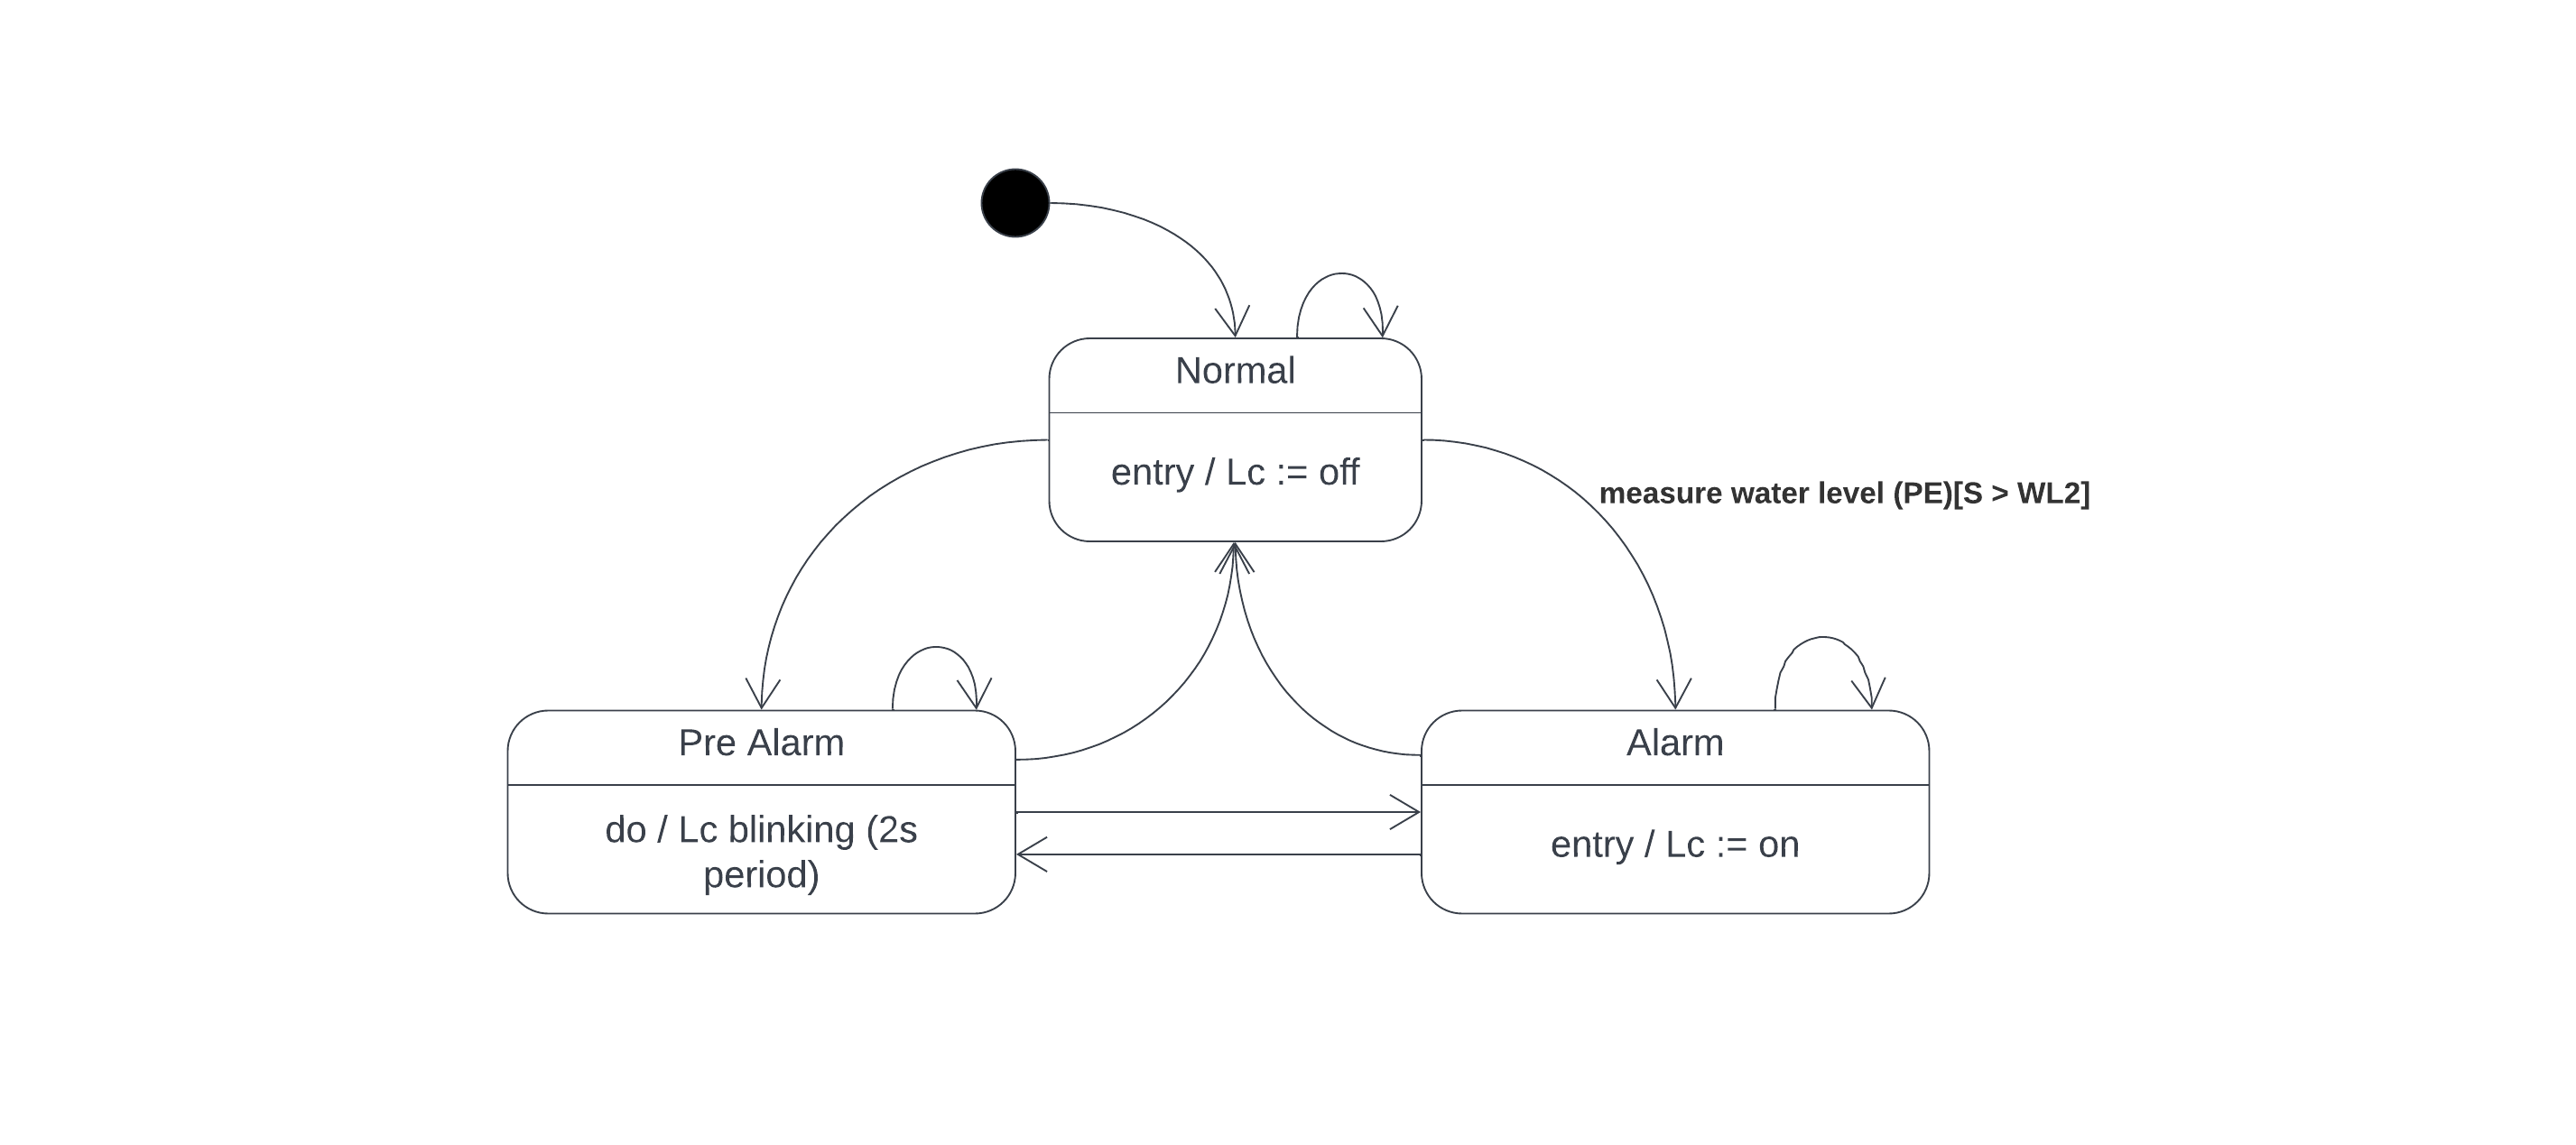
\includegraphics[width=\textwidth]{img/State - Blinking.png}
\caption{FSM Blinking led.}
\label{fig:FSMBlinking}
\end{figure}

\subsubsection{Manual Control task}
Questo task tiene internamente un bottone, la cui pressione mette alternatamente una variabile a true e false. Tramite la comunicazione diretta di questo task con ServoMotor task, quest'ultimo è in grado di capire quando dovrà farsi pilotare dal potenziometro e quando invece dal sonar.
Il diagramma degli stati è alquanto semplice poiché, come mostra la figura \ref{fig:FSMManual}, si compone di un solo stato in cui tale task è in ascolto di eventuali pressioni del bottone. Qualora queste avvengano la variabile ``manual'' viene messa a false se precedentemente a true o viceversa.

\begin{figure}[H]
\centering
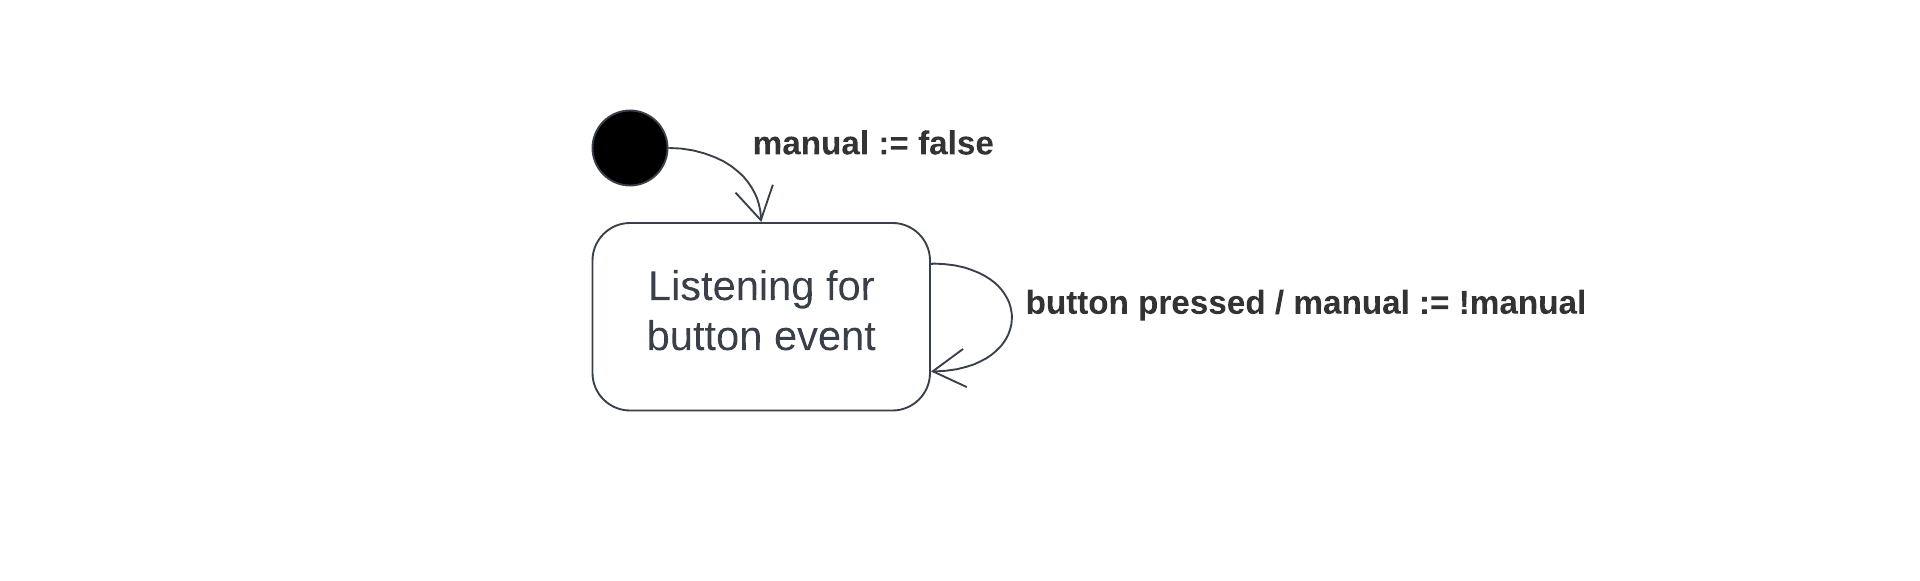
\includegraphics[width=\textwidth]{img/State - ManualTask.png}
\caption{FSM Manual Control task.}
\label{fig:FSMManual}
\end{figure}


\subsection{Pattern Observer}
In fase di implementazione è sorto il problema di come far comunicare i task fra loro. Per quanto detto fin'ora, infatti, l'interazione fra questi risulta di fondamentale importanza per il corretto funzionamento del sistema (Ad esempio il WaterLevel task necessità delle misure prese dal Sonar Task per valutare in che stato di allarme si trova, o ancora lo schermo lcd ha bisogno del water level task per capire se accendere o meno il display e quali, delle informazioni fornitegli da sonar e servo tasks, mostrare). 
La soluzione più banale a cui abbiamo pensato si basava sullo scambio di informazioni contenute in variabili globali. Questa strada, tuttavia, oltre ad essere poco flessibile risultava anche poco elegante. Tenendo conto anche del fatto che il flusso di esecuzione risulta difficilmente predicibile, dal momento che non è chiaro chi sovrascrive tali variabili e quando, abbiamo deciso di applicare il \emph{pattern Observer}. Esso è notevolmente vantaggioso perché
\begin{itemize}
    \item in un sistema embedded l'utilizzo delle risorse va tenuto in considerazione come fattore di primaria importanza. L'alternativa all'uso di variabili globali/oggetti condivisi sarebbe quello di fare polling di dati da parte di altri task.
    Con l'utilizzo di observer questa logica viene ribaltata facendo in modo che siano i task generatori di eventi (\emph{subjects}) ad avvisare gli interessati (\emph{observers}).
    \item Il flusso di esecuzione resta controllato poiché non vi sono variabili globali o oggetti condivisi modificabili e leggibili in qualunque momento da qualunque task. Solamente i subject, tramite la generazioni di eventi, comunicano dati rilevanti ai diretti interessati (che poi decideranno cosa farsene implementando il metodo \emph{update()}).
    \item Aggiungere funzionalità dipendenti da altre risulta facile poiché non è necessario creare un'interfaccia ad'hoc per la loro comunicazione. Sarà sufficiente iscrivere tali funzionalità ai soggetti generatori di eventi rilevanti per esse e implementare il metodo \emph{update()}.
\end{itemize}
Sebbene questo approccio abbia una serie di vantaggi indiscutibili, presenta anche un'evidente problematica. Facendo si che task terze eseguano porzioni di codice (in particolare quanto definito all'interno di \emph{update()}) di task, al di fuori dal periodo di esecuzione stabilito per essi dallo scheduler, si rompe la logica prevista dall'architettura basata su scheduling di task.
Questo, tuttavia, può essere un limite trascurabile nel momento in cui il contenuto di update() è costituito unicamente dalla scrittura di un dato che servirà quando lo scheduler attiverà lo specifico task aggiornato dal subject.
\subsubsection{Classe Event}
Ruolo di fondamentale importanza nell'architettura appena descritta è rappresentato dagli oggetti della classe \emph{Event}. Essi costituiscono il tramite fra Subjects e Observers.
\paragraph{Campi}
Poiché il tipo di dato memorizzato all'interno dell'evento dipende dalla natura del subject generatore, è stato inserito, all'interno della classe Event, un attributo che sfrutta il meccanismo dei \emph{template}(equivalente C++ dei generici in Java). Esso verrà specificato dal Subject al momento dell'effettiva istanziazione dell'evento.
Per alcuni Observer è sorto il problema di registrarsi a più Subject il cui evento era dello stesso tipo (Ad esempio l'LCD si è iscritto sia a ServoTask che a SonarTask, entrambi generanti eventi di tipo double). Per risolvere, oltre all'argomento dell'evento, è stato aggiunto un campo che rappresenta il tipo di Subject\footnote{Poiché Arduino non rende possibile l'uso di \emph{typeid} (analogo C++ della reflection in Java), si è deciso di utilizzare banalmente una enumerazione.}.

\paragraph{Problemi di memoria}
Poiché gli eventi sono oggetti generati a run-time, è sorto un problema di carenza di memoria che portava il sistema a bloccarsi e rientrare nel setup(). Dopo un'analisi alquanto travagliata siamo giunti alla conclusione che il problema insorgeva proprio dal momento che questa serie di oggetti veniva creato ma mai deallocato. La soluzione trovata è quella di cancellare l'evento una volta notificati tutti gli observers.  

Nella seguente figura \ref{fig:classidef} è rappresentato il diagramma delle classi nella versione implementata effettivamente. In essa è rappresentato solamente una delle varie interdipendenze Subject-Observer, nel caso di SonarTask-WaterTask.

\begin{figure}[H]
\centering
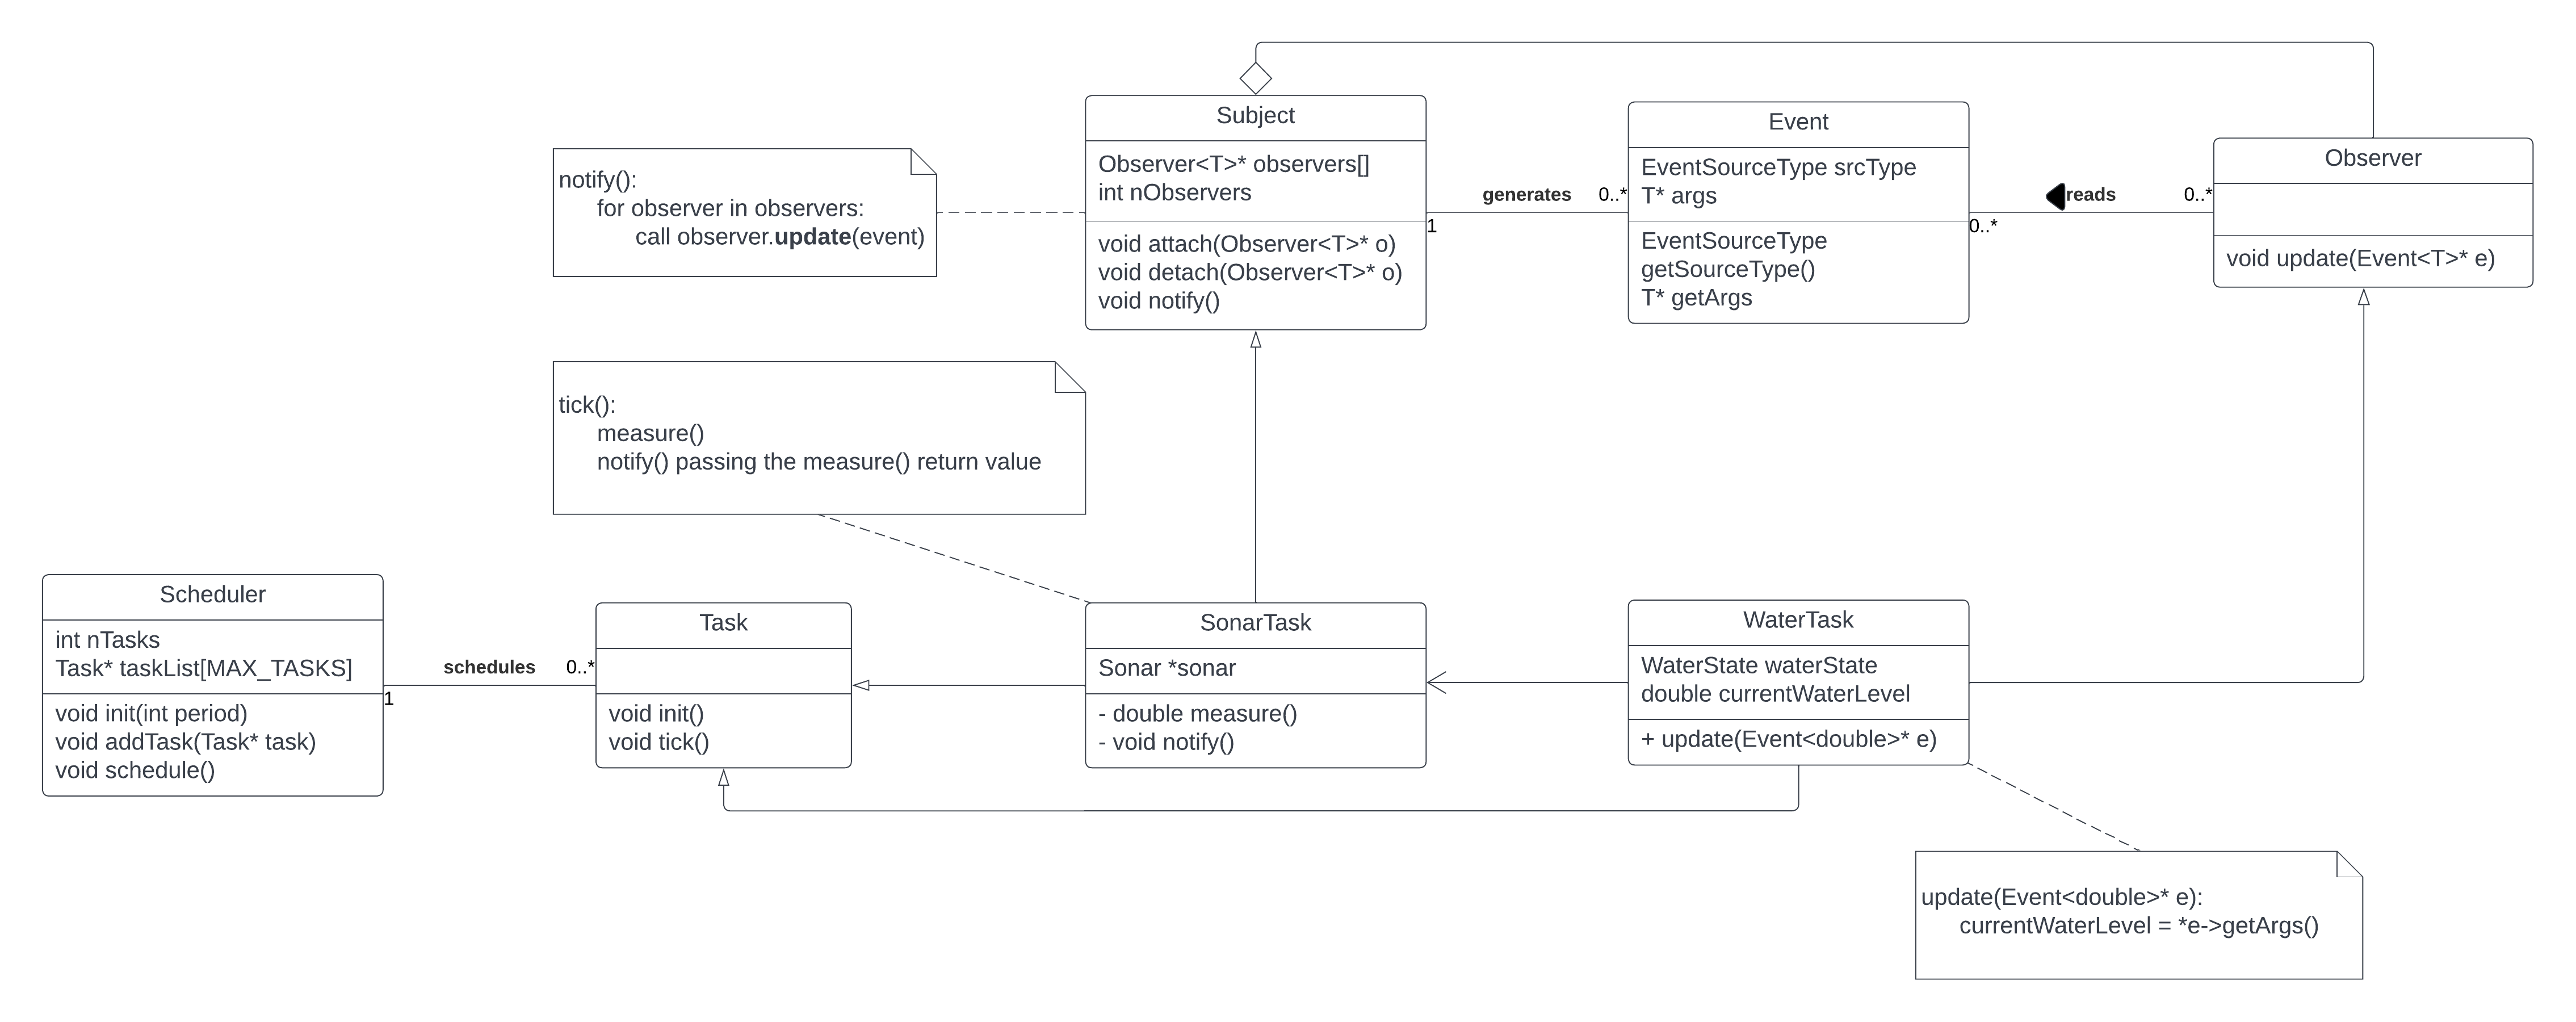
\includegraphics[width=1.1\textwidth]{img/Classi - Observer.png}
\caption{Class diagram SonarTask, WaterTask.}
\label{fig:classidef}
\end{figure}

\section{Adattamento run-time frequenza di campionamento}
Da specifiche risulta necessario adattare dinamicamente la frequenza di campionamento del sonar a seconda dello stato di allarme in vigore in un dato istante.
Per risolvere la questione è stato aggiunto un metodo alla classe task \emph{Task::updatePeriod(int)} che consente di aggiornare il periodo di attesa che lo scheduler aspetta prima di eseguire lo specifico task. Dal momento che quest'ultimo richiama il metodo \emph{Task::updateAndCheckTime(int)}, che al suo interno gestisce il periodo dello specifico task, prima di eseguire il suo tick(), non è necessario fare ulteriori modifiche affinché tutto funzioni.
\subsection{Come comunicare ai task quando cambiare periodo}
Il meccanismo utilizzato per far si che il sonar adatti il proprio periodo di tick è nuovamente basato sul pattern Observer. Il task del sonar si registra come observer di WaterTask il quale, a seguito di un cambiamento di stato, notifica il sonar stesso dell'evento. 
Questo principio, avendo predisposto le super classi \emph{Task}, \emph{Subject} e \emph{Observer}, può essere facilmente esteso a qualunque task si decidesse di adattare il periodo a run time.

\chapter{Wirings}
In questo capitolo viene mostrata la rappresentazione del cablaggio. Si è scelto di mantenere una suddivisione, anche a livello di cablaggio, che rispettasse per quanto possibile la suddivisione fatta a livello software. Dunque i sensori relativi ad un particolare task vengono mantenuti vicini.
\section{Descrizione dettagliata}
Il circuito è composto da due led verdi La e Lb, un led rosso Lc che si accenderà in caso di preallarme, un bottone B utilizzato per avere il controllo sulla valvola, un potenziometro Pot che serve per controllare l’apertura in gradi della valvola, un servo motore M che serve per aprire e chiudere le valvole che regolano il livello dell’acqua presente, un sonar S che è in grado di misurare la distanza da un oggetto situato di fronte ad esso, un Pir che misura la quantità di radiazioni infrarosse irradiate da un oggetto nel campo visivo del sensore, un sensore di luminosità(fotoresistenza) per controllare la quantità di luce presente e uno schermo LCD per stampare a video valori. 

\begin{figure}[H]
\centering
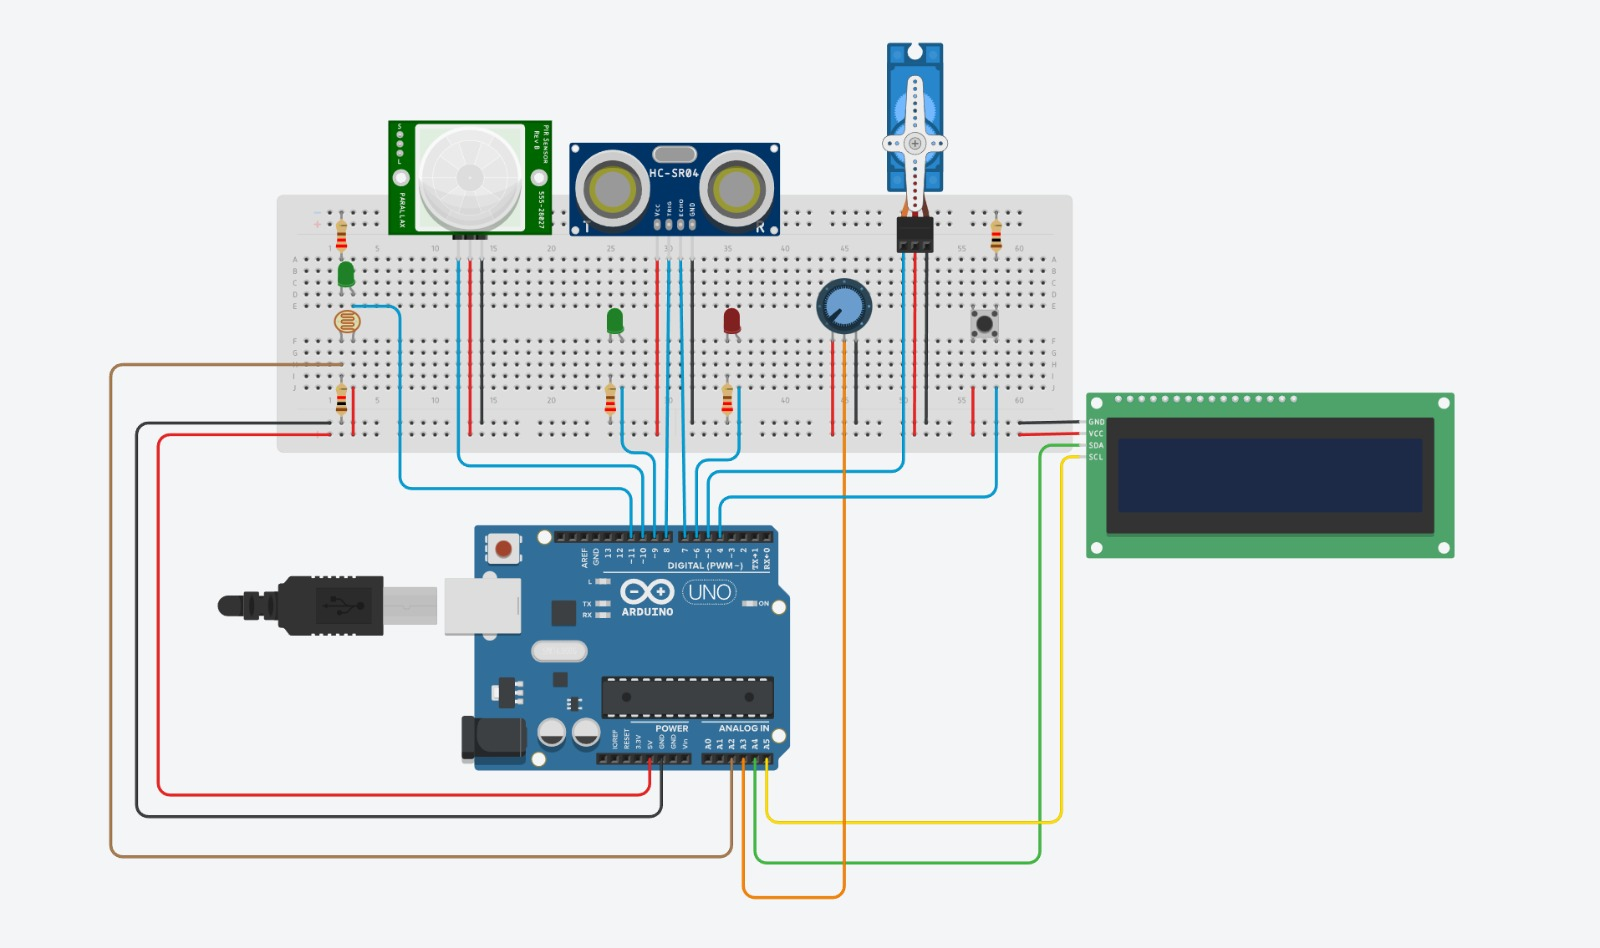
\includegraphics[width=\textwidth]{img/wirings.jpg}
\caption{Schema del cablaggio fatto su Thinkercad.}
\label{fig:wirings}
\end{figure}

\end{document}